\documentclass[../thesis.tex]{subfiles}

\begin{document}
\section {Xây dựng bộ tiêu chí đánh giá biến đổi KGKTCQ dưới ảnh hưởng NTM}
\subsection {Xây dựng Khung đánh giá không gian kiến trúc cảnh quan dứoi ảnh hưởng NTM}
Bộ tiêu chí được xây dựng dựa trên:
\begin{enumerate}
    \item \textbf{Bộ Tiêu Chí Quốc Gia Về Xã Nông Thôn Mới(491/QĐ-TTg) \& Bộ Tiêu Chí Quốc Gia Về Xã Nông Thôn Mới Giai Đoạn 2016 - 2020 (1980/QĐ-TTg)}: Hai bộ tiêu chí được thủ tướng ban hành để đánh giá quá trình xây dựng NTM tại các địa bàn trên hai giai đoạn. Trong Bảng tiêu chí, tôi lựa chọn các tiêu chí liên quan tới phát triển không gian kiến trúc cảnh quan để phục vụ công tác nghiên cứu đánh giá. Lý do tham khảo bộ tiêu chí này là do đây là khung tiêu chí hiện đang được áp dụng để đánh giá xây dựng NTM tại Việt Nam
    \item \textbf{LEED-ND-v4\cite{leed_v4}}: Bộ tiêu chí khu vực Bắc Mỹ LEED-ND được sử dụng trong việc đánh giá chứng chỉ khu ở bền vững. Lý do tham khảo bộ tiêu chí này là do (a) đây là bộ tiêu chí xây dựng hướng tới tính toàn cầu và (b) phổ biến trong chuyên ngành xây dựng.
    \item \textbf{RBESAS\cite{wan_ng_2016}}: (Rural Built Environmental Sustainability Assessment System). Bộ tiêu chí được các học giả Li và Ng sử dụng ban đầu để đánh giá chất lượng môi trường xây dựng các vùng nông thôn nghèo phía Đông Nam Trung Quốc. Lý do tham khảo bộ tiêu chí này là do (a) mục tiêu bộ tiêu chí hướng trực tiếp đến môi trường nông thôn và (b) vị trí tác giả áp dụng có vị trí địa lý gần với Việt Nam (c) bộ tiêu chí phổ biến trong giới nghiên cứu. 
    \item \textbf{Mô hình đánh giá 5D:\cite{ao_martek_2020}} 5 tiêu chí về mật độ, độ đa dạng, thiết kế, khoảng cách và khả năng tiếp cận được sử dụng phổ biến trong các nghiên cứu về không gian xây dựng (Built Environment). 
\end{enumerate}
\begin{longtable}{|p{1cm}|p{2cm}|p{3cm}|p{7cm}|}
\hline
\multicolumn{1}{|l|}{TT} &
  Mục &
  Tên tiêu chí &
  Nội dung tiêu chí \\ \hline
\endhead
%
1 &
  \multirow{3}{*}{Lập Quy hoạch} &
  \multirow{3}{*}{\begin{tabular}[c]{@{}l@{}}Lập Quy hoạch\\ (Tên cũ: Quy hoạch)\end{tabular}} &
  Nghiên cứu: Nghiên cứu và đánh giá/ so sánh hiện trạng/ phương án không gian kiến trúc cảnh quan trên quan điểm 5D, khoảng cách di chuyển, vật liệu địa phương, văn hóa tập quán, những chỉ tiêu tiêu chí tại địa phương, trong nước và trên thế giới \\ \cline{1-1} \cline{4-4} 
2 &
   &
   &
  Quy hoạch: Có quy hoạch chung xây dựng xã được phê duyệt và được công bố công khai đúng thời hạn \\ \cline{1-1} \cline{4-4} 
3 &
   &
   &
  Quản lý: Ban hành quy định quản lý quy hoạch chung xây dựng xã và tổ chức thực hiện theo quy hoạch \\ \hline
4 &
  \multirow{22}{*}{\begin{tabular}[c]{@{}l@{}}Quy hoạch\\ không gian\end{tabular}} &
  \multirow{5}{*}{\begin{tabular}[c]{@{}l@{}}Quy hoạch Khu ở mới\\ (tên tiêu chí cũ: \\Nhà ở dân cư)\end{tabular}} &
  Quy hoạch: Mật độ, tầng cao, hệ số sử dụng đất phù hợp với nhu cầu thực tiễn khu vực, quy chuẩn quốc gia, quy định khu vực, tham khảo các nghiên cứu về nhu cầu nhà ở trên thế giới \\ \cline{1-1} \cline{4-4} 
5 &
   &
   &
  Quy hoạch:Khu ở mới nằm trong khu vực có hạ tầng đảm bảo thuận lợi di chuyển tới trung tâm, tới khu lao động sản xuất, cấp điện, cấp thoát nước \\ \cline{1-1} \cline{4-4} 
6 &
   &
   &
  Quy hoạch: Vị trí xây dựng khu ở mới an toàn, không nằm trong vùng ngập thường xuyên, khu vực hay xảy ra bão lũ, độ dốc nhỏ tránh bị sạt lở \\ \cline{1-1} \cline{4-4} 
7 &
   &
   &
  Thiết kế: Nhà ở có thiết kế kiên cố, an toàn cho người sử dụng \\ \cline{1-1} \cline{4-4} 
8 &
   &
   &
  Thiết kế: Nhà ở thuận tiện cho người sử dụng được thiết kế hướng tới xanh sử dụng vật liệu địa phương, sử dụng hiệu quả vật liệu trong quá trình xây dựng \\ \cline{1-1} \cline{3-4} 
9 &
   &
  \multirow{5}{*}{\begin{tabular}[c]{@{}l@{}}Quy hoạch di chuyển\\ (tên tiêu chí cũ:\\ Giao thông)\end{tabular}} &
  Quy hoạch: Mạng lưới đường giao thông được phân cấp, được cứng hóa, phù hợp với nhu cầu di chuyển của người dân \\ \cline{1-1} \cline{4-4} 
10 &
   &
   &
  Quy hoạch: Quy hoạch mạng lưới giao thông với mật độ đường và mật độ nút giao thông hợp lý \\ \cline{1-1} \cline{4-4} 
11 &
   &
   &
  Quy hoạch: Bố trí các điểm trung chuyển, dừng của phương tiện giao thông có phễu tiếp cận phù hợp với người dân trong khu vực. \\ \cline{1-1} \cline{4-4} 
12 &
   &
   &
  Thiết kế: Thiết kế hướng tới các đối tượng tham gia giao thông, có tuyến đi bộ/xe đạp liền mạch \\ \cline{1-1} \cline{4-4} 
13 &
   &
   &
  Thiết kế: Thiết kế những tuyến phố có kiến trúc được quy định (độ rộng mặt đứng, chiều cao so với bề rộng mặt đường) thân thiện với người đi bộ/ đi xe đạp. \\ \cline{1-1} \cline{3-4} 
14 &
   &
  \multirow{3}{*}{\begin{tabular}[c]{@{}l@{}}Quy hoạch \\ Hạ tầng kỹ thuật\end{tabular}} &
  Giao thông: Các tuyến đường được thiết kế tuân thủ quy chuẩn tiêu chuẩn bộ GTVT, có tham khảo đề xuất các thiết kế hiệu quả, tối ưu trên thế giới \\ \cline{1-1} \cline{4-4} 
15 &
   &
   &
  Thủy lợi: Hệ thống kênh mương, đường ống cấp thoát nước được thiết kế tuân thủ quy chuẩn, tiêu chuẩn trong nước, có tham khảo đề xuất các thiết kế hiệu quả, tối ưu trên thế giới \\ \cline{1-1} \cline{4-4} 
16 &
   &
   &
  Xử lý chất thải: \\ \cline{1-1} \cline{3-4} 
17 &
   &
  \multirow{4}{*}{\begin{tabular}[c]{@{}l@{}}Quy hoạch\\ Khu trung tâm\end{tabular}} &
  Quy hoạch: Quy hoạch khu trung tâm và các hạ tầng xã hội đảm bảo khả năng tiếp cận của người dân, kết nối với hạ tầng hiện trạng, kết hợp nghiên cứu các hạ tầng xã hội hiện trạng và khu vực lân cận, tránh quy hoạch thừa. Phân chia sử dụng đất, mật độ, tầng cao, hệ số sử dụng đất hợp lý, nén, tránh lãng phí tài nguyên đất. \\ \cline{1-1} \cline{4-4} 
18 &
   &
   &
  Thiết kế: Trường học: Tỷ lệ trường học các cấp: mầm non, mẫu giáo, tiểu học, trung học cơ sở có cơ sở vật chất và thiết bị dạy học đạt chuẩn quốc gia. Bố trí các trường các cấp thuận tiện với khả năng di chuyển người dân khu vực. Có nghiên cứu chọn lọc các mô hình kiến trúc tiên tiến trên thế giới để áp dụng. \\ \cline{1-1} \cline{4-4} 
19 &
   &
   &
  Thiết kế: Cơ sở vật chất văn hóa: Bố trí nhà thi đấu và nhà văn hóa xã thuận tiện với khả năng di chuyển người dân khu vực. Có nghiên cứu chọn lọc các mô hình kiến trúc tiên tiến trên thế giới để áp dụng. \\ \cline{1-1} \cline{4-4} 
20 &
   &
   &
  Thiết kế: Cơ sở hạ tầng thương mại nông thôn: Bố trí chợ thuận tiện với khả năng di chuyển người dân khu vực. Xác định quy mô chợ phù hợp với nhu cầu sử dụng. Có nghiên cứu chọn lọc các mô hình kiến trúc tiên tiến trên thế giới để áp dụng. \\ \cline{1-1} \cline{3-4} 
21 &
   &
  \multirow{3}{*}{\begin{tabular}[c]{@{}l@{}}Quy hoạch\\ Không gian xanh\end{tabular}} &
  Quy hoạch: Cân đối chỉ tiêu diện tích không gian xanh/ người đảm bảo phát triển bền vững. \\ \cline{1-1} \cline{4-4} 
22 &
   &
   &
  Quy hoạch: Phân bố không gian xanh phù hợp với khoảng cách đi lại của người sử dụng \\ \cline{1-1} \cline{4-4} 
23 &
   &
   &
  Thiết kế: Các không gian xanh thiết kế mở, đa dạng về quy mô liên kết với hệ thống giao thông, hệ thống công trình công cộng để tăng tính liền mạch cho khu vực nghiên cứu; đồng thời đóng vai trò là những không gian sinh thái khu vực \\ \cline{1-1} \cline{3-4} 
24 &
   &
  \multirow{2}{*}{\begin{tabular}[c]{@{}l@{}}Quy hoạch \\ bảo tồn cảnh quan,\\ cảnh quan mặt nước,\\ không gian sản xuất Nông nghiệp\end{tabular}} &
  Quy hoạch: Không xây dựng trong những khu vực cảnh quan ngập nước, nước mặt. Những khu vực trong vùng phụ cận hạn chế mật độ và độ cao xây dựng \\ \cline{1-1} \cline{4-4} 
25 &
   &
   &
  Quy hoạch: Hạn chế xây dựng trong những khu vực sản xuất nông nghiệp năng suất cao, tuân thủ theo quy hoạch sản xuất nông nghiệp \\ \hline
\end{longtable}
\subsection {Xây dựng bộ tiêu chí đánh giá Không gian KTCQ dưới ảnh hưởng NTM tại khu vực nghiên cứu}
\begin{landscape}
\begin{longtable}{|p{2cm}|p{2cm}|p{2cm}|p{5cm}|p{6cm}|}
\hline
\multicolumn{3}{|p{6cm}|}{Các tiêu chí} &
  \multicolumn{1}{p{5cm}|}{Nội dung} &
  \multicolumn{1}{p{6cm}|}{Tham khảo} \\ \hline
\endhead
%
\multicolumn{1}{|c|}{\multirow{3}{*}{Lập Quy hoạch}} &
  \multicolumn{1}{c|}{\multirow{3}{*}{\begin{tabular}[c]{@{}c@{}}Lập Quy hoạch\\ (Tên cũ: Quy hoạch)\end{tabular}}} &
  \textit{1.1. Nghiên cứu} &
  Nghiên cứu quy hoạch cấp trên, quy hoạch tổng thể phát triển kinh tế - xã hội khu vực, hiện trạng dân cư, kinh tế, văn hóa, xã hội, sử dụng đất, hiện trạng hạ tầng cơ sở. &
  \begin{tabular}[c]{@{}l@{}}NĐ 44/2015\\ TT 02/2017\end{tabular} \\ \cline{3-5} 
\multicolumn{1}{|c|}{} &
  \multicolumn{1}{c|}{} &
  1.2. Quy hoạch &
  Lập quy hoạch theo đúng quy hoạch hiện hành &
  TCVN 4454:2012 \par  4. Quy định chung \par  5. Quy hoạch xây dựng xã nông thôn mớiNĐ 44/2015 \par  Mục 3. QUY HOẠCH XÂY DỰNG NÔNG THÔNTT 02/2017 \par  Điều 8. Nội dung hồ sơ đồ án quy hoạch chung xây dựng xã \par  Điều 20. Nội dung công bố quy hoạch xây dựng nông thônTT 21/2009 \par  Điều 5. Lập quy hoạch xây dựng nông thôn. \par  Điều 6. Đồ án điều chỉnh quy hoạch xây dựng nông thôn. \par  Điều 7. Lấy ý kiến đối với đồ án quy hoạch xây dựng nông thôn.\\ \cline{3-5} 
\multicolumn{1}{|c|}{} &
  \multicolumn{1}{c|}{} &
  1.3. Quản lý &
  Ban hành quy định quản lý quy hoạch chung xây dựng xã và tổ chức thực hiện theo quy hoạch &
  NĐ 44/2015 \par  TT 02/2017 \par  Điều 21. Quy định quản lý và cung cấp thông tin quy hoạch xây dựng nông thôn \par  QCVN 21/2009: \par  Điều 3. Quản lý quy hoạch xây dựng nông thôn.QCVN 14/2009: \par  Chương VIII. Các quy định về quản lý\\ \hline
\multirow{21}{*}{\begin{tabular}[c]{@{}l@{}}Quy hoạch\\ Không gian\end{tabular}} &
  \multicolumn{1}{c|}{\multirow{3}{*}{\begin{tabular}[c]{@{}c@{}}1. Quy hoạch Khu ở mới\\ (tên tiêu chí cũ: Nhà ở dân cư)\end{tabular}}} &
  1.1. Quy hoạch: Chỉ tiêu sử dụng đất &
  Quy định các thông số dựa trên cơ sở thống kê và so sánh các hệ số hợp lý cho khu ở đáng sốngChỉ tiêu xây dựng: \par  Mật độ xây dựng:  \par  Tầng cao: \par  Hệ số sử dụng đất: &
 6.1.1. Quy mô dân số và đất để xây dựng mới và mở rộng các điểm dân cư nông thôn \par  6.1.1.5- 6.1.1.6 \par  Bảng 1 - Chỉ tiêu đất xây dựng điểm dân cư nông thôn \par  Phụ lục B. Diện tích đất ở và hình thái kiến trúc nhà ở theo vùng miền/ B.2. Đối với vùng đồng bằng sông Hồng \par  LEED ND: \par  NPD Prerequisite: Compact Development \par  NPD Credit: Compact Development. \par  QCVN-14-2009: \par  Bảng 1 \par  Tổng điều tra dân số và nhà ở 2019 \par Nông thôn: 3.6 người/ hộ \par  Đồng Bằng Sông Hồng: 3,4 người/ hộ \par  Hà Nội: 3.6 người/ hộ \\ \cline{3-5} 
 &
  \multicolumn{1}{c|}{} &
  1.2. Quy hoạch:Vị trí xây dựng &
   Không nằm trên các khu vực nhạy cảm sinh học, dễ tổn thương \par  2) Đảm bảo thuận tiện tiếp cận tới khu vực làm việc và công cộng \par  3) Không lạm dụng đất nông nghiệp thành khu ở \par  4) Đảm bảo hệ thống mạng lưới điểm dân cư, khoảng cách từ khu ở tới khu vực canh tác \par  5) Đảm bảo được bài toán nhu cầu hiện tại và trong tương lai &
    2.4. Quy hoạch khu ở  \par  TCVN 4454:2012 \par  6.1.1. Quy mô dân số và đất để xây dựng mới và mở rộng các điểm dân cư nông thôn \par  6.1.1.1 - 6.1.1.4 \par  6.1.2. 6.1.2. Yêu cầu đối với khu ởLLC: \par  IMPERATIVE 01: LIMITS TO GROWTHLeed ND:  \par  SMART LOCATION AND LINKAGE (SLL)/SMART LOCATION  \par  SMART LOCATION AND LINKAGE (SLL)/SLL CREDIT: PREFERRED LOCATIONS\\ \cline{3-5} 
 &
  \multicolumn{1}{c|}{} &
  1.3. Thiết kế: Nhà ở &
    Nhà ở bền vững \par  2) Nhà ở sử dụng năng lượng hiệu quả \par  3) Nhà ở hướng tới yếu tố xanh &
  TCVN 4454:2012: \par  Phụ lục B. Diện tích đất ở và hình thái kiến trúc nhà ở theo vùng miền/ B.2. Đối với vùng đồng bằng sông Hồng \par  LOTUS-Homes \\ \cline{2-5} 
 &
  \multicolumn{1}{c|}{\multirow{5}{*}{\begin{tabular}[c]{@{}c@{}}2.Quy hoạch di chuyển\\ (tên tiêu chí cũ: Giao thông)\end{tabular}}} &
  2.1. Quy hoạch: Phân cấp giao thông &
  Đường đã được phân cấp theo chức năng và lưu lượng sử dụng chưa &
   5.3.2. Quy hoạch giao thông \par  TCVN 10380:2014: \par  4.2. Hệ thống đường GTNT được phân thành 4 cấp kỹ thuật A, B, C và D...  không có ô tô chạy qua. \par  Bảng 4.Tổng hợp phân cấp kỹ thuật đường GTNT theo chức năng của đường \\ \cline{3-5} 
 &
  \multicolumn{1}{c|}{} &
  2.2. Quy hoạch: Mật độ giao thông &
    Mật độ điểm nút (nút/km2) \par Mật độ đường giao thông trong khu vực (km/km2) &
   Human Scale and Humane PlacesLeed ND \par  NPD PREREQUISITE: CONNECTED AND OPEN COMMUNITY  \par  NPD CREDIT: CONNECTED AND OPEN COMMUNITY  \par Samaeul Undong: \par  Farm roads\\ \cline{3-5} 
 &
  \multicolumn{1}{c|}{} &
  2.3. Quy hoạch: Quy hoạch hệ thống giao thông công cộng &
  \begin{tabular}[c]{@{}l@{}}Các điểm chờ xe buýt\\ Bến trung chuyển\end{tabular} &
  Leed ND:\par LT CREDIT: ACCESS TO QUALITY TRANSIT\par LLC:\par IMPERATIVE 16: UNIVERSAL ACCESS TO COMMUNITY SERVICES \\ \cline{3-5} 
 &
  \multicolumn{1}{c|}{} &
  2.4. Quy hoạch: Mạng lưới đường đi bộ, đi xe đạp &
  Mạng lưới đường đi bộ/ xe đạp đã liền mạch, khuyến khích người sử dụng chưa &
  Leed ND:NPD PREREQUISITE: WALKABLE STREETS\par NPD CREDIT: WALKABLE STREETS \par NPD CREDIT: CONNECTED AND OPEN COMMUNITY \\ \cline{3-5} 
 &
  \multicolumn{1}{c|}{} &
  2.5. Thiết kế: Thiết kế tuyến phố &
  Thiết kế tuyến phố thân thiện với người đi bộ, đi xe đạp &
  LLC:Human Scale and Humane Places\par Leed ND: \par NPD PREREQUISITE: WALKABLE STREETS\par NPD CREDIT: WALKABLE STREETS \\ \cline{2-5} 
 &
  \multirow{4}{*}{\begin{tabular}[c]{@{}l@{}}3.Quy hoạch \\ Hạ tầng kỹ thuật\end{tabular}} &
  3.1. Giao thông: Yêu cầu kỹ thuật giao thông &
  Công trình đã đáp ứng chức năng/ thẩm mĩ; đảm bảo an toàn chưa &
  TCVN 10380:2014\par TCVN 4054:2005\\ \cline{3-5} 
 &
   &
  3.2. Thủy lợi: Yêu cầu kỹ thuật công trình thủy lợi &
  Công trình đã đáp ứng chức năng/ thẩm mĩ; đảm bảo an toàn chưa &
  TCVN 8423 : 2010 \\ \cline{3-5} 
 &
   &
  3.3. Cấp điện: Yêu cầu kỹ thuật công trình cấp điện và thông tin &
  Công trình đã đáp ứng chức năng/ thẩm mĩ; đảm bảo an toàn chưa &
   \\ \cline{3-5} 
 &
   &
  3.4. Xử lý chất thải, nước thải và nghĩa trang: Yêu cầu kỹ thuật xử lý nước thải chất thải rắn, nghĩa trang &
  Công trình đã đáp ứng chức năng/ thẩm mĩ; đảm bảo an toàn chưa &
   \\ \cline{2-5} 
 &
   \multirow{5}{*}{\begin{tabular}[c]{@{}l@{}}Quy hoạch\\ Khu trung tâm\end{tabular}} &
  4.1. Quy hoạch: Chỉ tiêu xây dựng & Đảm bảo chỉ tiêu, đáp ứng chức năng khu trung tâm &
Hạ tầng kỹ thuật  Bảng 1 \par TCVN 4454:2012\par Bảng 1 - Chỉ tiêu đất xây dựng điểm dân cư nông thôn \\ \cline{3-5} 
 &
   &
  4.2. Quy hoạch: Trung tâm xã &
  Dễ dàng tiếp cận với người dân khu vực &
  LEED ND: \par NPD CREDIT: WALKABLE STREETS \par QCVN 14/2009:\par 2.5. Quy hoạch khu trung tâm xã \\ \cline{3-5} 
 &
   &
  4.3. Thiết kế: Trường học &
  Dễ dàng tiếp cận với người dân khu vực \par Đảm bảo các tiêu chí xây dựng công trình giáo dục &
  NPD CREDIT: NEIGHBORHOOD SCHOOLS\par TCVN 4454:2012 \par 6.1.3.3. Trường học \\ \cline{3-5} 
 &
   &
  4.4. Thiết kế: Cơ sở vật chất văn hóa &
  Thân thiện\par Dễ dàng tiếp cận với người dân khu vực\par Gắn liền với không gian xanh, không gian công cộng &
  LLC:Human Scale and Humane Places\par Leed ND: NPD PREREQUISITE: WALKABLE STREETS\par NPD CREDIT: WALKABLE STREETS \par TCVN 4454:2012\par 6.1.3.5. Cơ sở vật chất văn hóa - thể thao \\ \cline{3-5} 
 &
   &
  4.5. Thiết kế: Cơ sở hạ tầng thương mại nông thôn &
  Dễ dàng tiếp cận với người dân khu vực &
  LLC:Human Scale and Humane Places\par Leed ND: NPD PREREQUISITE: WALKABLE STREETS\par NPD CREDIT: WALKABLE STREETS \par TCVN 4454:20126.1.3.6. Chợ\par QCVN 14/2009:2.5. Quy hoạch khu trung tâm xã \\ \cline{2-5} 
 &
  \multirow{3}{*}{\begin{tabular}[c]{@{}l@{}}Quy hoạch\\ Không gian xanh\end{tabular}} &
  5.1. Quy hoạch: Chỉ tiêu xây dựng &
   &
  QCVN-14-2009:\par Bảng 1\par TCVN 4454:2012Bảng 1 - Chỉ tiêu đất xây dựng điểm dân cư nông thôn \\ \cline{3-5} 
 &
   &
  5.2. Quy hoạch: Phân bố không gian cây xanh mặt nước &
   &
  NPD CREDIT: ACCESS TO CIVIC AND PUBLIC SPACE \\ \cline{3-5} 
 &
   &
  5.3. Thiết kế: Thiết kế không gian xanh hướng tới sinh thái &
   &
   \\ \cline{2-5} 
 &
  \multirow{2}{*}{\begin{tabular}[c]{@{}l@{}}Quy hoạch\\ sản xuất nông nghiệp\end{tabular}} &
  6.1. Quy hoạch: Phân bố không gian sản xuất nông nghiệp &
   &
   \\ \cline{1-1} \cline{3-5} 
 &
   &
  6.2. Thiết kế: Công trình phục vụ không gian sản xuất &
   &
   \\ \hline
   \end{longtable}
\end{landscape}

\subsection {Tham khảo ý kiến chuyên gia}
\section {Đánh giá biến đổi KGKTCQ dưới ảnh hưởng NTM tại khu vực nghiên cứu}
\subsection {Tiêu chí Lập Quy hoạch:}
\subsubsection {Tiêu chí Lập Quy hoạch: Nghiên cứu}
Hai quy hoạch được lập vào hai bối cảnh khác nhau, bởi vậy chúng chịu ảnh hưởng bởi :\\
\textbf{DA2009:} Trong ĐỀ ÁN XÂY DỰNG NÔNG THÔN MỚI CẤP XÃ (Mô hình nông thôn mới giai đoạn 2009 – 2011) (DA2009) \cite{da2009}, QHC NTM Xã Thụy Hương được xây dựng trên cơ sở:

 \begin{quote}
 \begin{itemize}
\item "Nghị quyết 26/TƯ ngày 05/8/2008 của Ban Chấp hành Trung ương Khoá X về nông nghiệp, nông dân, nông thôn.
\item Thông báo 238-TB/TƯ ngày 07/4/2009 của Ban Bí thư về chương trình xây dựng thí điểm mô hình nông thôn mới trong thời kỳ đẩy mạnh CNH - HĐH;
\item Quyết định số 491/2009/QĐ-TTg ngày 16/4/2009 của Thủ tướng Chính phủ về ban hành Bộ tiêu chí quốc gia nông thôn mới.
\item Công văn số 1416/ BNN-KTHT ngày 27/5/2009 của Bộ Nông nghiệp \& PTNT về việc hướng dẫn thực hiện xây dựng đề án thí điểm mô hình nông thôn mới cấp xã.
\item Các thông tư, hướng dẫn thực hiện xây dựng mô hình nông thôn mới của các Bộ, Ngành có liên quan.”
\end{itemize}
 \end{quote}

Như vậy, DA2009 được thành lập trên cơ sở thí điểm việc thực hiện NTM.

\textbf{DCQH2017:} Trong khi đó, DCQH2017 được xây dựng trên cơ sở CTMTQGVNTM đã được đi vào hoạt động và các QH cấp trên ảnh hưởng:
\begin{itemize}
\item Chương trình mục tiêu Quốc gia về xây dựng Nông thôn mới của Chính phủ và các đồ án quy hoạch cấp trên khác được duyệt.  
\item Quy hoạch chung xây dựng Thủ đô Hà Nội đến năm 2030 tầm nhìn đến năm 2050
\item Quy hoạch chung xây dựng huyện Chương Mỹ đến năm 2030
\item Quy hoạch chung Thị trấn sinh thái Chúc Sơn đến năm 2030, tỷ lệ 1/5.000\\ 
\end{itemize}
\textbf{Kết luận:} Có thể nhận thấy hai QHC xây dựng huyện Chương Mỹ ảnh hưởng lớn tới các trục phát triển (hình 5.2) \citation{qhcxdchuongmy} trong khi đó QHC Thị trấn Sinh thái Chúc Sơn có ảnh hưởng lớn đến ranh giới hành chính của xã (hình 5.1) \citation{qd505}\\
\clearpage

\begin{figure}
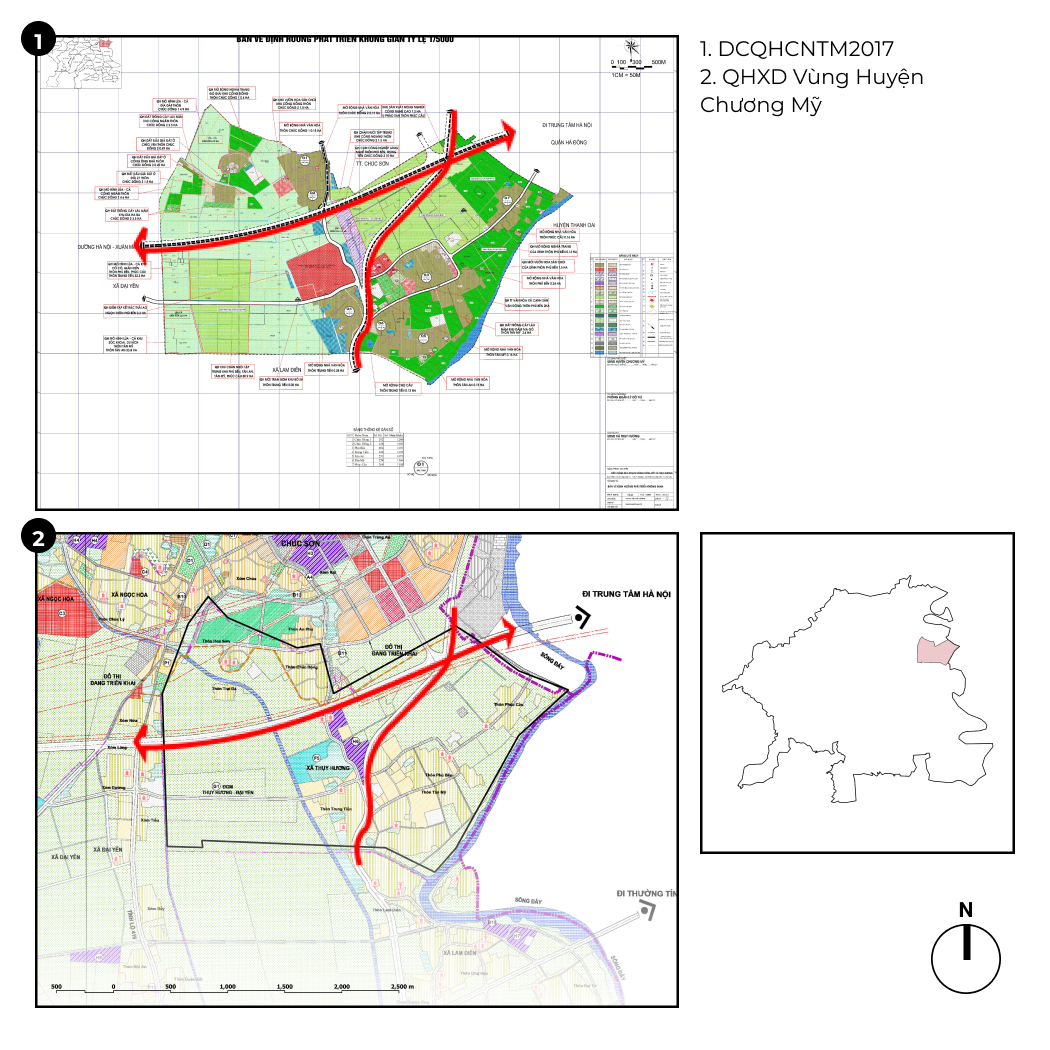
\includegraphics[width=15cm]{TC1.1.jpg}\caption{So sánh QHCNTM và QHC xây dựng vùng huyện Chương Mỹ}
\end{figure}

\begin{figure}[h!]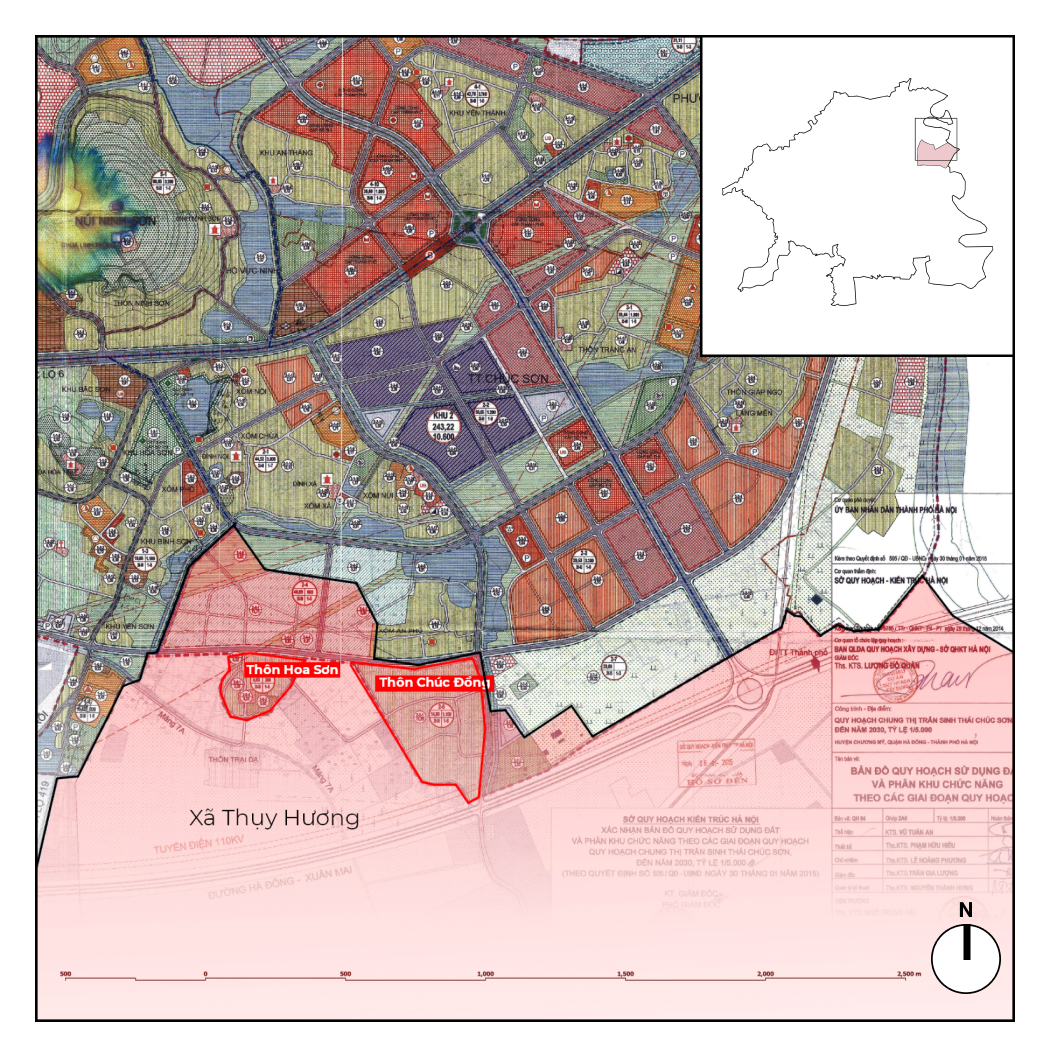
\includegraphics[width=15cm]{TC1.1-1.jpg}
\caption{QHC NTM xã Thụy Hương trong QHC Thị trấn Sinh thái Chúc Sơn}
\end{figure}

\subsubsection {Tiêu chí Lập Quy hoạch: Quy hoạch}
\begin{landscape}
\begin{longtable}{ | m{3cm} | m{18cm}| } 
\hline
Tên &ĐỀ ÁN XÂY DỰNG NÔNG THÔN MỚI CẤP XÃ (Mô hình nông thôn mới giai đoạn 2009 – 2011) \\
\hline
Phạm vi và ranh giới &Xã Thụy Hương \\
\hline
Mục tiêu &- Đầu tư nâng cấp cơ sở hạ tầng: \par - Phấn đấu tới 2011 thực chất xây dựng được xã Thuỵ Hương cơ bản đạt tiêu chí mô hình nông thôn mới thời kỳ CNH - HĐH, thể hiện các đặc trưng: kinh tế bước đầu phát triển, đời sống vật chất, tinh thần được nâng cao, hình thức sản xuất phù hợp, hướng tới phát triển nông nghiệp công nghệ cao với phát triển nhanh TTCN và dịch vụ, của vùng nông thôn mới ven đô. Xã hội nông thôn ổn định, giàu bản sắc văn hoá dân tộc, dân trí nâng cao, môi trường sinh thái được bảo vệ, các tổ chức trong hệ thống chính trị vững mạnh. \par - Trở thành một bài học cho những khu vực trong ĐBCT Sông Hồng \\
\hline
Tác động chính & 1. \textbf{Giao thông:}tiếp tục đầu tư xây dựng hệ thống đường giao thông nông thôn, hệ thống đường giao thông nội đồng.
- Đường trục xã: cần bê tông hóa 4,58 km còn lại. 
- Đường trục thôn: cần bê tông hóa 2,9 km còn lại và bổ sung 7 km đường chưa có rãnh thoát nước\par - Đường ngõ xóm: bê tông hóa 3,97 km còn lại và bổ sung 4,5 km đường ngõ chưa có rãnh thoát nước\par - Đường nội đồng: tổng 10.4 km cần cứng hoá.\par - Hệ thống cầu (trên đường nội đồng): cần đầu tư thay thế 2 cầu cũ. \\& \textbf{2. Thuỷ lợi:}\par - Cải tạo nâng cấp một số trạm bơm (trước mắt cải tạo trạm bơm Trại Tằm).\par - Kiên cố 5,33 km kênh tưới.\par - Cải tạo, nâng cấp 90 cống và 03 cầu.\\&  \textbf{3. Hệ thống điện:}\par - Cải tạo nâng cấp một số trạm biến áp hiện nay không đáp ứng yêu cầu điện phục vụ sản xuất và sinh hoạt của nhân dân.\par - Nâng cấp một số tuyến đường cao thế, hạ thế đã xuống cấp, không an toàn.\par - Bổ sung hệ thống chiếu sáng công cộng.\par - Công tác quản lý và kinh doanh điện: bàn giao cho ngành điện. \\&  \textbf{4. Trường học:}\par - Nâng cấp cải tạo, xây mới một số phòng học ở khu trung tâm để đảm bảo đạt chuẩn.\par - Nâng cấp cải tạo, xây mới một số phòng chức năng đáp ứng yêu cầu dạy và học, cơ bản đạt tiêu chí.\par - Nâng cấp cải tạo các khu bổ trợ (khu hiệu bộ, nhà để xe, nhà vệ sinh…)\par - Quy hoạch, xây dựng chỉnh trang khuôn viên trường (sân trường, cổng, tường rào, vườn hoa…) \\&  5. Cơ sở hạ tầng Y tế:\par - Nâng cấp, cải tạo các công trình y tế hiện có\par - Xây dựng mới 01 khu điều trị\par - Bổ sung một số trang thiết bị y tế phục vụ cho khám, chữa bệnh\par - Quy hoạch, chỉnh trang hệ thống sân, vườn cây thuốc, khuôn viên \\&\textbf{ 6. Cơ sở vật chất văn hoá:}\par - Cải tạo nâng cấp: \par + 01 nhà văn hoá thôn Tân An. \par + Đầu tư thiết bị (tủ sách, nối mạng internet…) cho 07 nhà văn hoá thôn. \par+ Nâng cấp, trùng tu các di tích đã được xếp hạng, lăng mộ danh nhân Lê Ngô Cát, chùa Hoa Sơn… \par+ Tu bổ, tôn tạo 01 nghĩa trang liệt sỹ.\par - Xây dựng mới: \par+ 01 nhà văn hoá thôn Trung Tiến \par+ Đầu tư hệ thống các công trình thể thao và mua sắm dụng cụ thể thao. \\&  \textbf{7. Chợ:} Cải tạo nâng cấp chợ hiện có đảm bảo trao đổi hàng hoá cho nhân dân trong khu vực. Thúc đẩy sản xuất phát triển, tạo điều kiện để ngành dịch vụ tăng nhanh.\\&  \textbf{8. Nhà ở dân cư nông thôn:}\par - Nâng cấp, xây mới 04 nhà đã xuống cấp, hư hỏng nặng.\par - Hỗ trợ chỉnh trang một số nhà ở không phù hợp với quy hoạch và kiểu dáng kiến trúc của khu vực nông thôn.\par - Hỗ trợ để tôn tạo, bảo tồn một số nhà truyền thống, nhà cổ. \\&  \textbf{9. Sản xuất nông nghiệp:}\par + Xây dựng vùng sản xuất Rau an toàn: diện tích canh tác khoảng 80 ha tại khu vực bãi, gồm các xứ đồng: Quai Xanh, Rặng Xoan, Ụ Pháo, Cửa Đình. (triển khai ngay cuối năm 2009). Xây dựng vùng sản xuất hoa, cây cảnh: diện tích khoảng 10 ha tại khu Chỉ Bộ (lập xong quy hoạch trong năm 2009). \par+ Xây dùng vùng sản xuất Cây ăn quả: diện tích canh tác 40 ha (bưởi diễn, nhãn muộn, cam canh…), quy hoạch ở các xứ đồng: trại Tằm; bờ sông (Phúc Cầu, Tân An, Phú Bõn…). Quy hoạch các khu nuôi trồng thủy sản tập trung kết hợp với chăn nuôi gia súc, gia cầm, trồng cây ăn quả theo hướng đa canh, đa mục tiêu. Tổng diện tích 30,1 ha tại khu đồng Du Kích, khu Ổ Gà. Quy hoạch chăn nuôi tập trung xa khu dân cư: quy mô 30 ha vùng bãi, tập trung vào bò sữa, bò thịt, gà; chủ yếu tận dụng thức ăn xanh. \\&  \textbf{10. Tiểu thủ công nghiệp: }Đầu tư xây dựng điểm công nghiệp làng nghề tập trung khoảng 5-10 ha, trước mắt đến 2011 đầu tư khoảng 3-5 ha tại khu Đám Mạ (Trung Tiến, Phú Bến, Phúc Cầu). \\&  \textbf{11. Dịch vụ thương mại:} Quy hoạch một số khu sinh thái gắn với du lịch dịch vụ (khu hồ trung tâm xã, khu bãi ven sông Đáy…), kêu gọi các doanh nghiệp vào đầu tư.\\
\hline
\end{longtable}
\clearpage
\begin{longtable}{ | m{3cm} | m{18cm}| } 
\hline
Tên &\textbf{Đồ án điều chỉnh quy hoạch chung xây dựng nông thôn mới xã Thụy Hương, huyện Chương Mỹ đến năm 2020, tầm nhìn đến năm 2030.}\\
\hline
Phạm vi và ranh giới & Xã Thụy Hương   \\ \hline
Mục tiêu    &1. Cụ thể hóa QH cấp cao \par2. Phát triển KT- XH khu vực trên tiêu chí hiện đại, giữ gìn bản sắc, bền vững, nâng cao chất lượng đời sống nhân dân, thu hẹp khoảng cách tới cuộc sống đô thị. \par3. Cải tạo các hạ tầng cần thiết \par4. Đề xuất các dự án ưu tiên \par5. Xây dựng Quy định quản lý theo đồ án Quy hoạch chung xây dựng xã    \\ \hline
Tác động chính    &Cập nhật QH Trung tâm văn hóa – thể dục thể thao chăm sóc sức khỏe cộng đồng Khu ủy ban xã Thôn Phú Bến, Phúc Cầu, Trung Tiến diện tích khoảng 20ha lấy vào đất trồng cây lâu năm và đất nuôi trồng thủy sản, đất lúa; \par -  Bổ sung quy hoạch khoảng 0,1ha đất trụ sở ban chỉ quy quân sự xã sau UBND xã lấy vào đất nuôi trồng thủy sản; \par -  Bổ sung quy hoạch sân chơi, vườn hoa tại khu Cổng Đồng, thôn Chúc Đồng 2 với diện tích khoảng 1,8ha. \\&\textbf{ 1. Quy hoạch phát triển khu trung tâm:} Điều chỉnh mở rộng quy hoạch trung tâm xã và điểm dân cư nông thôn xã Thụy Hương với quy mô khoảng 25ha. \\& \textbf{2. Quy hoạch phát triển các điểm dân cư:}Điều chỉnh, bổ sung quy hoạch đất ở nông thôn phát triển mới\\& 3.\textbf{ Điều chỉnh, bổ sung quy hoạch sản xuất nông nghiệp:}\par - Quy hoạch vùng đất trang trại tổng hợp \par - Quy hoạch vùng đất trồng cây ăn quả;\par - Quy hoạch đất lúa – cá \\& \textbf{4.Quy hoạch sản sản xuất công nghiệp, thương mại dịch vụ:} \par -  Cập nhật quy hoạch cụm công nghiệp Thụy Hương với diện tích khoảng 11,04ha theo Quy hoạch chung của huyện. \par -  Cập nhật quy hoạch khu sản xuất nông nghiệp công nghệ cao gắn du lịch trải nghiệm nông nghiệp tại khu Ụ Pháo San, thôn Phúc Cầu với diện tích 7,2ha. \par -  Bổ sung quy hoạch điểm tập kết vật liệu xây dựng với diện tích 0,64ha tại khu Bờ San, thôn Phú Bến lấy vào đất nuôi trồng thủy sản. \\& \textbf{5. Hệ thống đường giao thông:}Cập nhật quy hoạch hệ thống đường giao thông theo quy hoạch chung huyện Chương Mỹ đi qua địa bàn xã Thụy Hương gồm có. \par -  Đường Xuân Mai – Hà Nội qua xã có chiều dài 4,24km, có bề rộng mặt cắt ngang đường B=73,5m. \par -  Đường huyện quy hoạch qua xã có chiều dài 3,02km, có bề rộng mặt cắt ngang đường B=42m. \par -  Đường đê Hữu Đáy đoạn từ thôn An Phú, thị trấn Chúc Sơn đến ngã 3 (đường vào UBND xã Thụy Hương và đường đê hữu Đáy) qua xã có chiều dài 1,5km, có bề rộng mặt cắt ngang đường B=25÷30m. \par -  Tuyến đường liên xã đoạn từ UBND xã Thụy Hương đến xã Đại Yên có chiều dài 2,24km, có bề rộng mặt cắt ngang đường B=30m. \par -  Các tuyến đường liên xã đi có bề rộng mặt cắt ngang đường B=14m. Đường liên thôn có bề rộng mặt cắt ngang đường B=6÷10m; đường ngõ xóm có bề rộng mặt cắt ngang đường B=5÷5,5m. \\& \textbf{6. Quy hoạch nghĩa trang, nghĩa địa:} \par -  Điều chỉnh quy hoạch đất nghĩa trang khu Rặng Xoan, thôn Tân An với diện tích 2,8ha sang đất trồng rau an toàn; \par -  Điều chỉnh mở rộng nghĩa trang Gò Giải, khu Sát Gạo, thôn Chúc Đồng 1 thêm 0,4ha lấy vào đất bằng trồng cây hàng năm; \\&\textbf{ 7. Quy hoạch thoát nước thải và vệ sinh môi trường} \par -  Bổ sung vào Quy hoạch mới điểm tập kết rác thải sinh hoạt tại vị trí Khu Ao Ngọn, diện tích 0,1ha ở Thôn Phú Bến, lấy vào đất nuôi trồng thủy sản; 10. Danh mục các dự án ưu tiên theo kỳ kế hoạch để đạt tiêu chí nông thôn mới \par -  Nâng cấp trạm bơm. \par -  Đầu tư nâng cấp một số tuyến kênh tưới tiêu chính. \par -  Đầu tư nâng cấp các tuyến nội đồng chính. \par -  Hỗ trợ các dự án phát triển sản xuất. \par -  Đầu tư hệ thống rãnh thoát nước thuộc khu dân cư các thôn, xóm trên địa bàn xã    \\
\hline
\end{longtable}
\end{landscape}

\begin{table}[h!]
\centering
\begin{tabular}{ | m{7.5cm} | m{7.5cm}| } 
\hline      
\multicolumn{1}{|c|}{\textbf{DA2009}}& \multicolumn{1}{c|}{\textbf{DCQHC2017}} \\
\hline  
Trong 11 hạng mục có ảnh hưởng tới KGKTCQ trong DA2009 của xã Thụy Hương, có: \par - 3 hạng mục về QH Hạ tầng  \par - 4 hạng mục về QH Hạ tầng xã hội\par  - 1 hạng mục về QH Nhà ở \par - 3 hạng mục về QH Phát triển Kinh tế \par Đề án được xây dựng trong thời gian ngắn, tầm nhìn ngắn hạn (2009 – 2010) nên tập trung chủ yếu vào bổ sung các hạ tầng hiện trạng, ít xây mới với mục tiêu bổ sung các hạ tầng còn thiếu sót để hoàn thành mục tiêu NTM, làm bài học cho những khu vực lân cận. &Trong DCQHC2017, có 7 hạng mục có ảnh hưởng tới KGKTCQ: \par - 1 hạng mục QH Khu trung tâm  \par - 1 hạng mục QH Điểm dân cư nông thôn  \par - 2 hạng mục QH Phát triển Kinh tế  \par - 3 hạng mục về QH Hạ tầng  \par Đề án được xây dựng với tầm nhìn 10 năm, thừa hưởng một số định hướng từ QH cấp cao, mục tiêu phát triển kinh tế, cải thiện đời sống xã hội, hướng tới chất lượng cuộc sống đô thị. \\
\hline 
\end{tabular}
\end{table}

\textbf{Kết luận:} Trên cơ sở những phân tích trên, có thể nhận thấy DA2009 tập trung vào bổ sung những hạ tầng còn thiếu, trong khi đó DCQHC2017 tập trung vào đồng bộ hạ tầng với QHXD cấp cao hơn. Dựa trên QC 21/2009/TT-BXD về "Quy định việc lập, thẩm định, phê duyệt và quản lý
quy hoạch xây dựng nông thôn", 2 đồ án đã cơ bản tuân thủ các nội dung của QHC NTM.Tuy nhiên trong DA2009, một vài nội dung chưa được làm rõ. Đối chiếu với các nội dung trong "Điều 5. Lập quy hoạch xây dựng nông thôn" về "Nội dung quy hoạch xây dựng mạng lưới điểm dân cư nông thôn" Mục 1 và Mục 3 có thể thấy DA2009 chưa "Bố trí mạng lưới điểm dân cư nông thôn tập trung" mà mới chỉ cải thiện chất lượng công trình hiện tại. Trong khi đó DCQHC2017 đã thể hiện rõ nội dung này thông qua mục "Quy hoạch phát triển các điểm dân cư".\\
\subsubsection {Tiêu chí Lập Quy hoạch: Quản lý}

\begin{table}[h!]
\centering
\begin{tabular}{ | m{7.5cm} | m{7.5cm}| } 
\hline      
\multicolumn{1}{|c|}{\textbf{DA2009}}& \multicolumn{1}{c|}{\textbf{DCQHC2017}} \\
\hline  
Hình thành BAN QUẢN LÝ CHƯƠNG TRÌNH XÂY DỰNG THÍ ĐIỂM MÔ HÌNH NÔNG THÔN MỚI tại địa phương đảm bảo thực hiện theo đúng đề án. &Đưa ra quyết định ban hành quy định quản lý xây dựng theo Đồ án điều chỉnh Quy hoạch chung xây dựng nông thôn mới xã Thụy Hương, huyện Chương Mỹ đến năm 2020, tầm nhìn đến năm 2030 \\
\hline 
\end{tabular}
\end{table}

\textbf{Kết luận:} DA2009 và DCQHC2017 đều có giải pháp để quản lý QHXD khu vực nghiên cứu.
\clearpage

\subsection {Quy hoạch Khu ở mới}
\subsubsection{Quy hoạch: Chỉ tiêu sử dụng đất}

\subsubsection{Quy hoạch:Vị trí xây dựng}
\begin{table}[h!]
\centering
\begin{tabular}{ | m{3cm} | m{12cm}| } 
\hline  
Thực tế 2019 & Những điểm dân cư hiện trạng phân bố tập trung dạng co cụm, xung quanh những điểm thôn hiện có. \\
\hline 
DA2009 & DA2009 bổ sung các điểm dân cư mới xung quanh khu trung tâm tại thôn Trung Tiến và Phú Điền- thuận tiện tiếp cận HTXH.
\\
\hline 
DCQHC2017 & DCQHC2017 các điểm dân cư QH phân tán tại thôn Trung Tiến và ven thôn Chúc Đồng\\
\hline 
\end{tabular}
\end{table}


\begin{figure}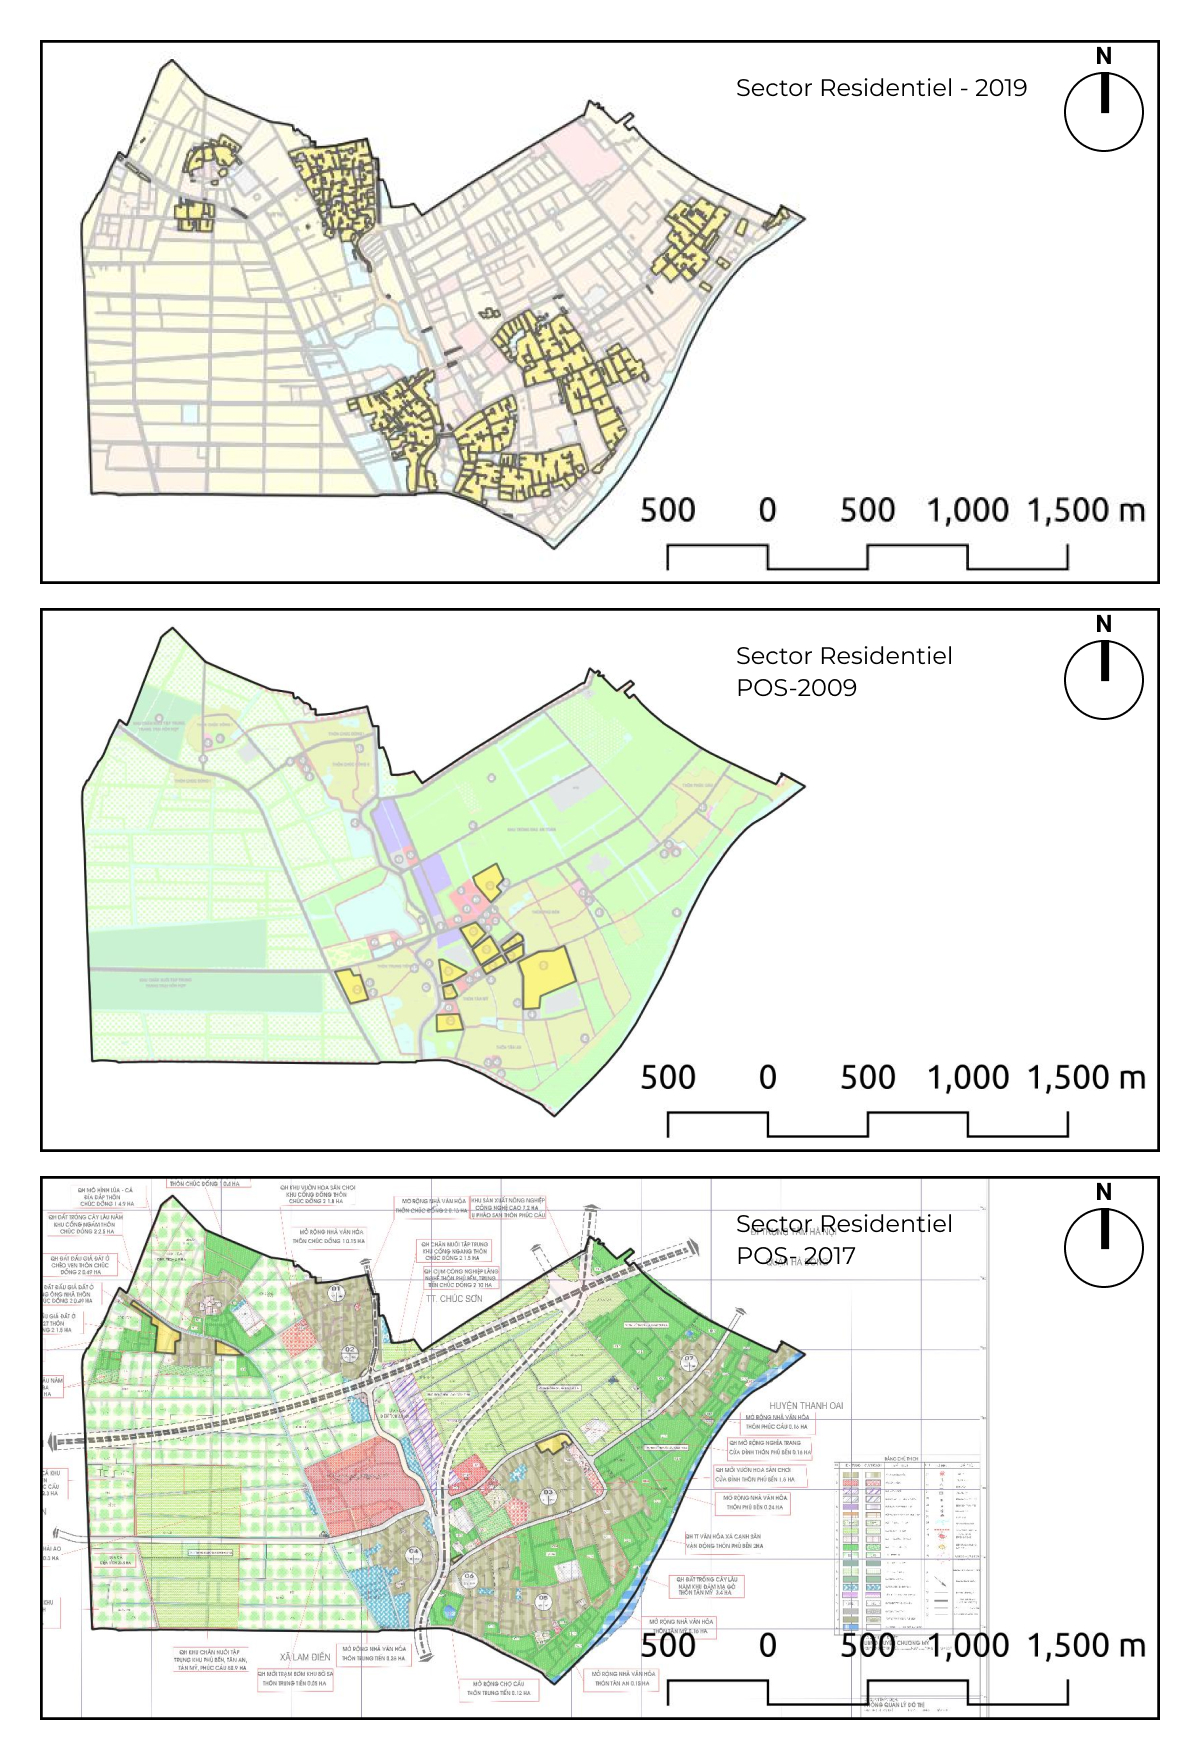
\includegraphics[width=15cm]{Sector-Residentiel.jpg}\caption{Khu ở qua các bản đồ}\end{figure}
\clearpage

\subsection {Quy hoạch di chuyển}
\begin{table}
\centering
\begin{tabular}{ | m{3cm} | m{12cm}| } 
\hline  
Thực tế 2019 & Hệ thống giao thông bám theo hệ thống đê Hữu Đáy, các đường bờ vùng bờ thửa. \\
\hline 
DA2009 & DA2009 bổ sung hai trục giao thông cơ giới lớn từ Tây Nam ĐÔng Bắc, kết hợp với Khu Công nghiệp và Khu chăn nuôi mới được quy hoạch.
\\
\hline 
DCQHC2017 & DCQHC2017 tổ chức hệ thống giao thông lớn giao cắt qua xã, ngăn chia các thôn, trục Xuân Mai Hà Nội đi qua đình của xã, có thể ảnh hưởng tới không gian cảnh quan xung quanh đình làng.\\
\hline 
\end{tabular}
\end{table}
\begin{figure}\caption{Khu ở qua các bản đồ}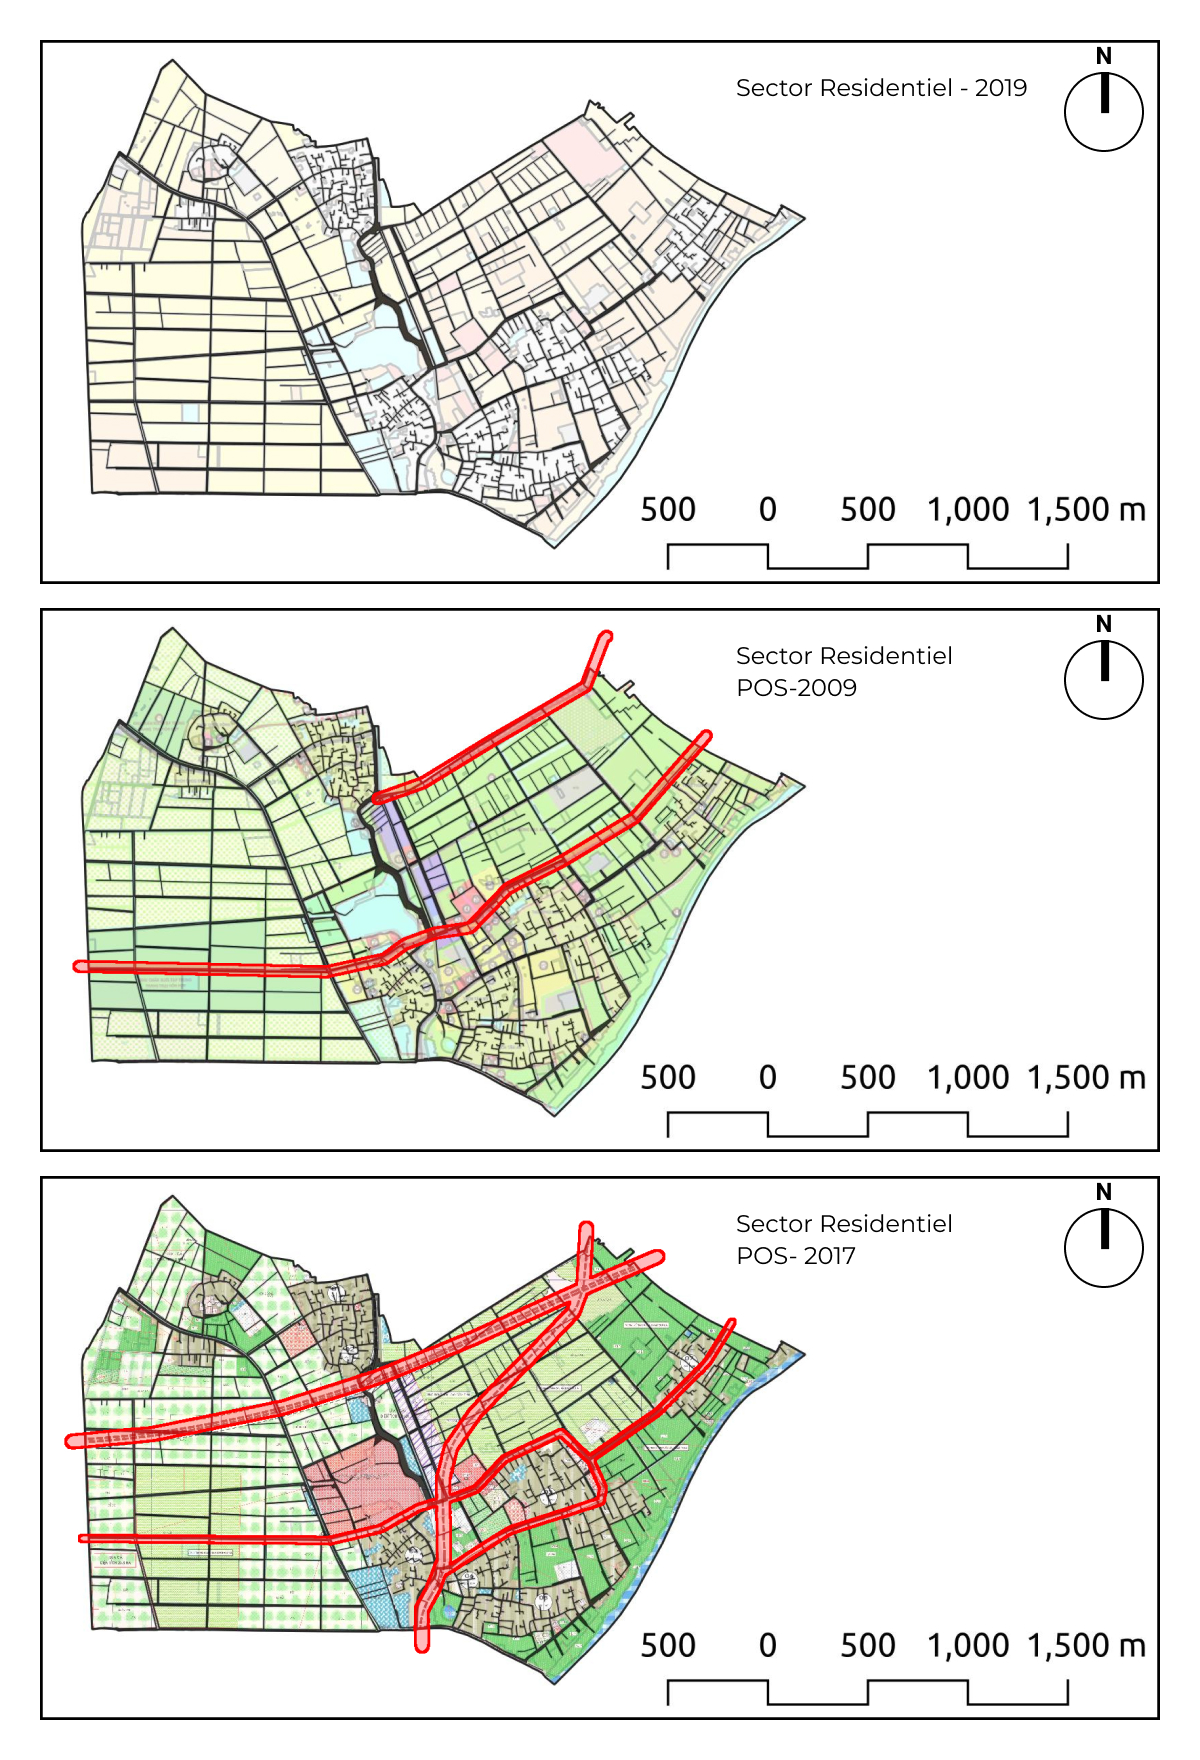
\includegraphics[width=15cm]{Graphic/TC3.jpg}\end{figure}
\clearpage

\subsection {Quy hoạch Hạ tầng kỹ thuật}

\subsection {Quy hoạch Khu trung tâm}
\begin{figure}
\caption{Đánh giá Quy hoạch phân bố HTXH}
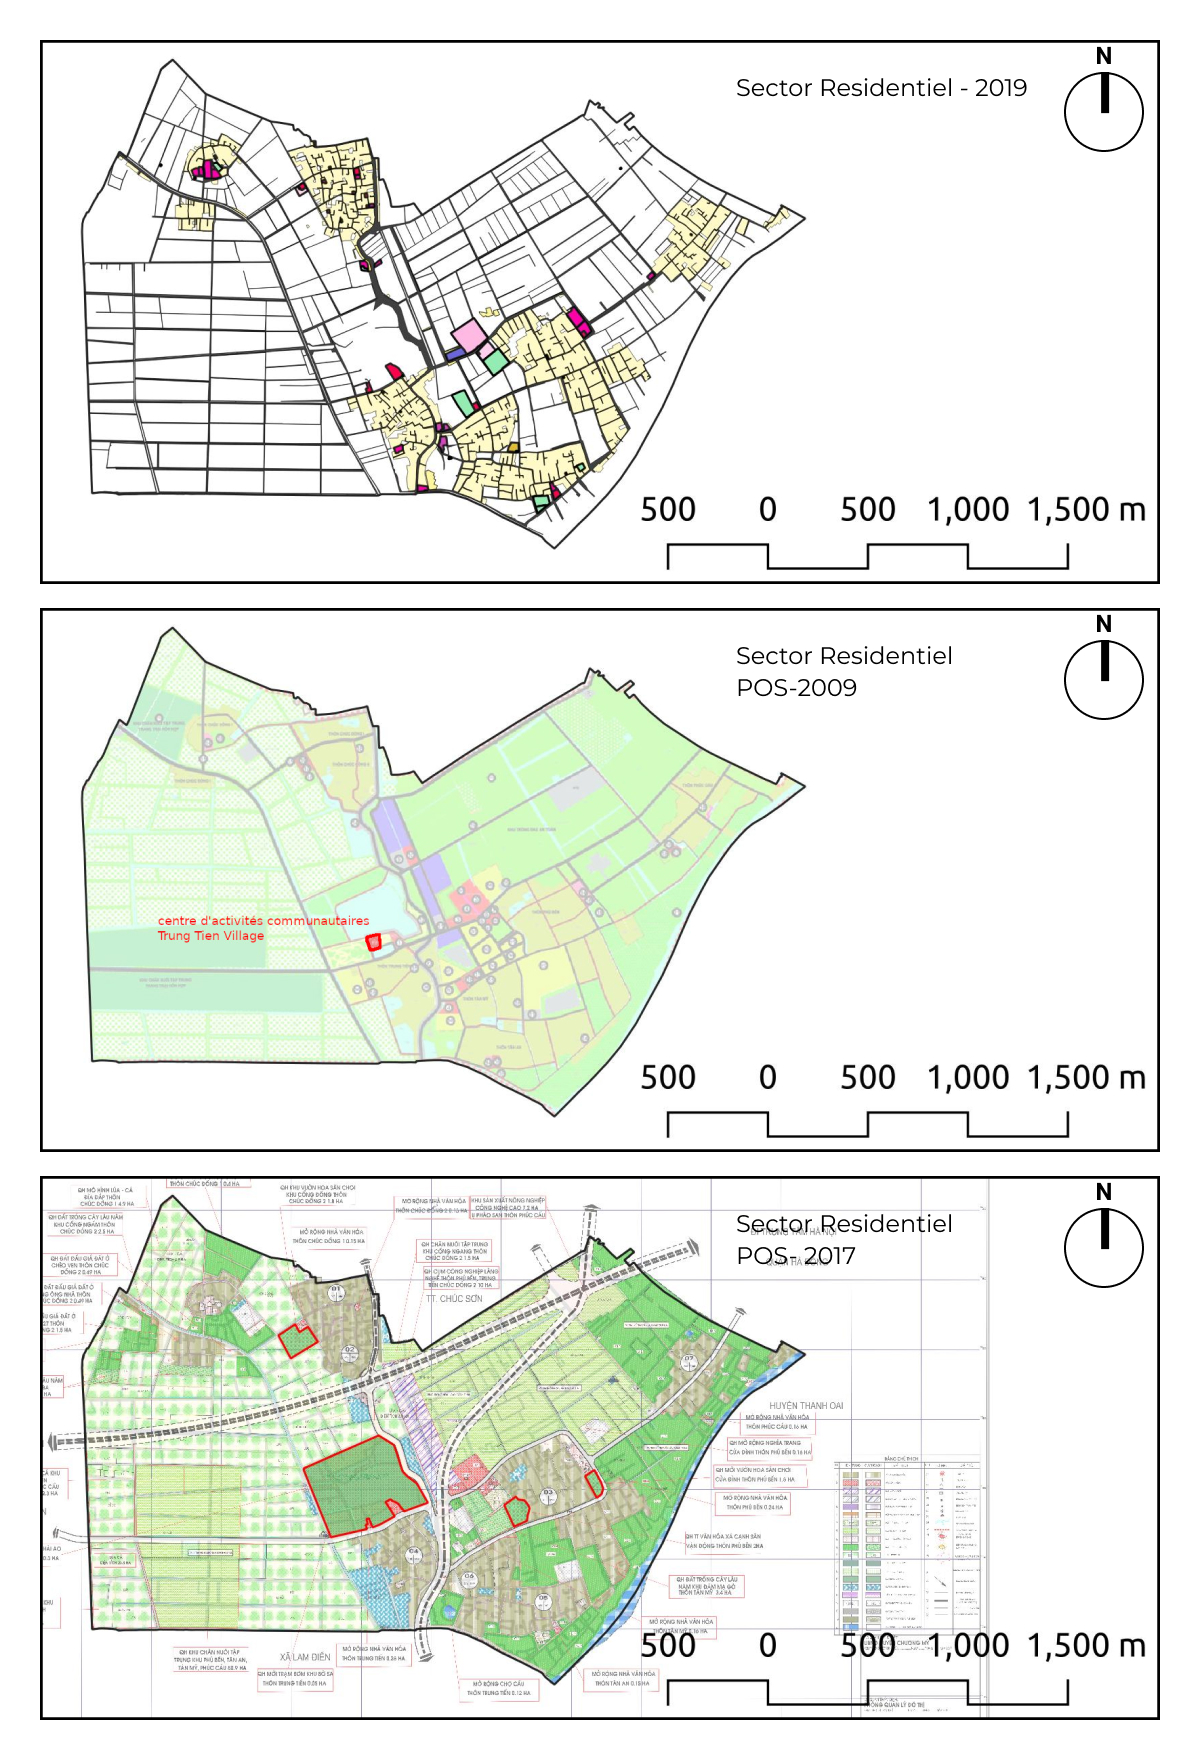
\includegraphics[width=15cm]{Graphic/TC5-QH-KTT.jpg}
\end{figure}
\clearpage
\subsection {Quy hoạch Không gian xanh}

\begin{figure}
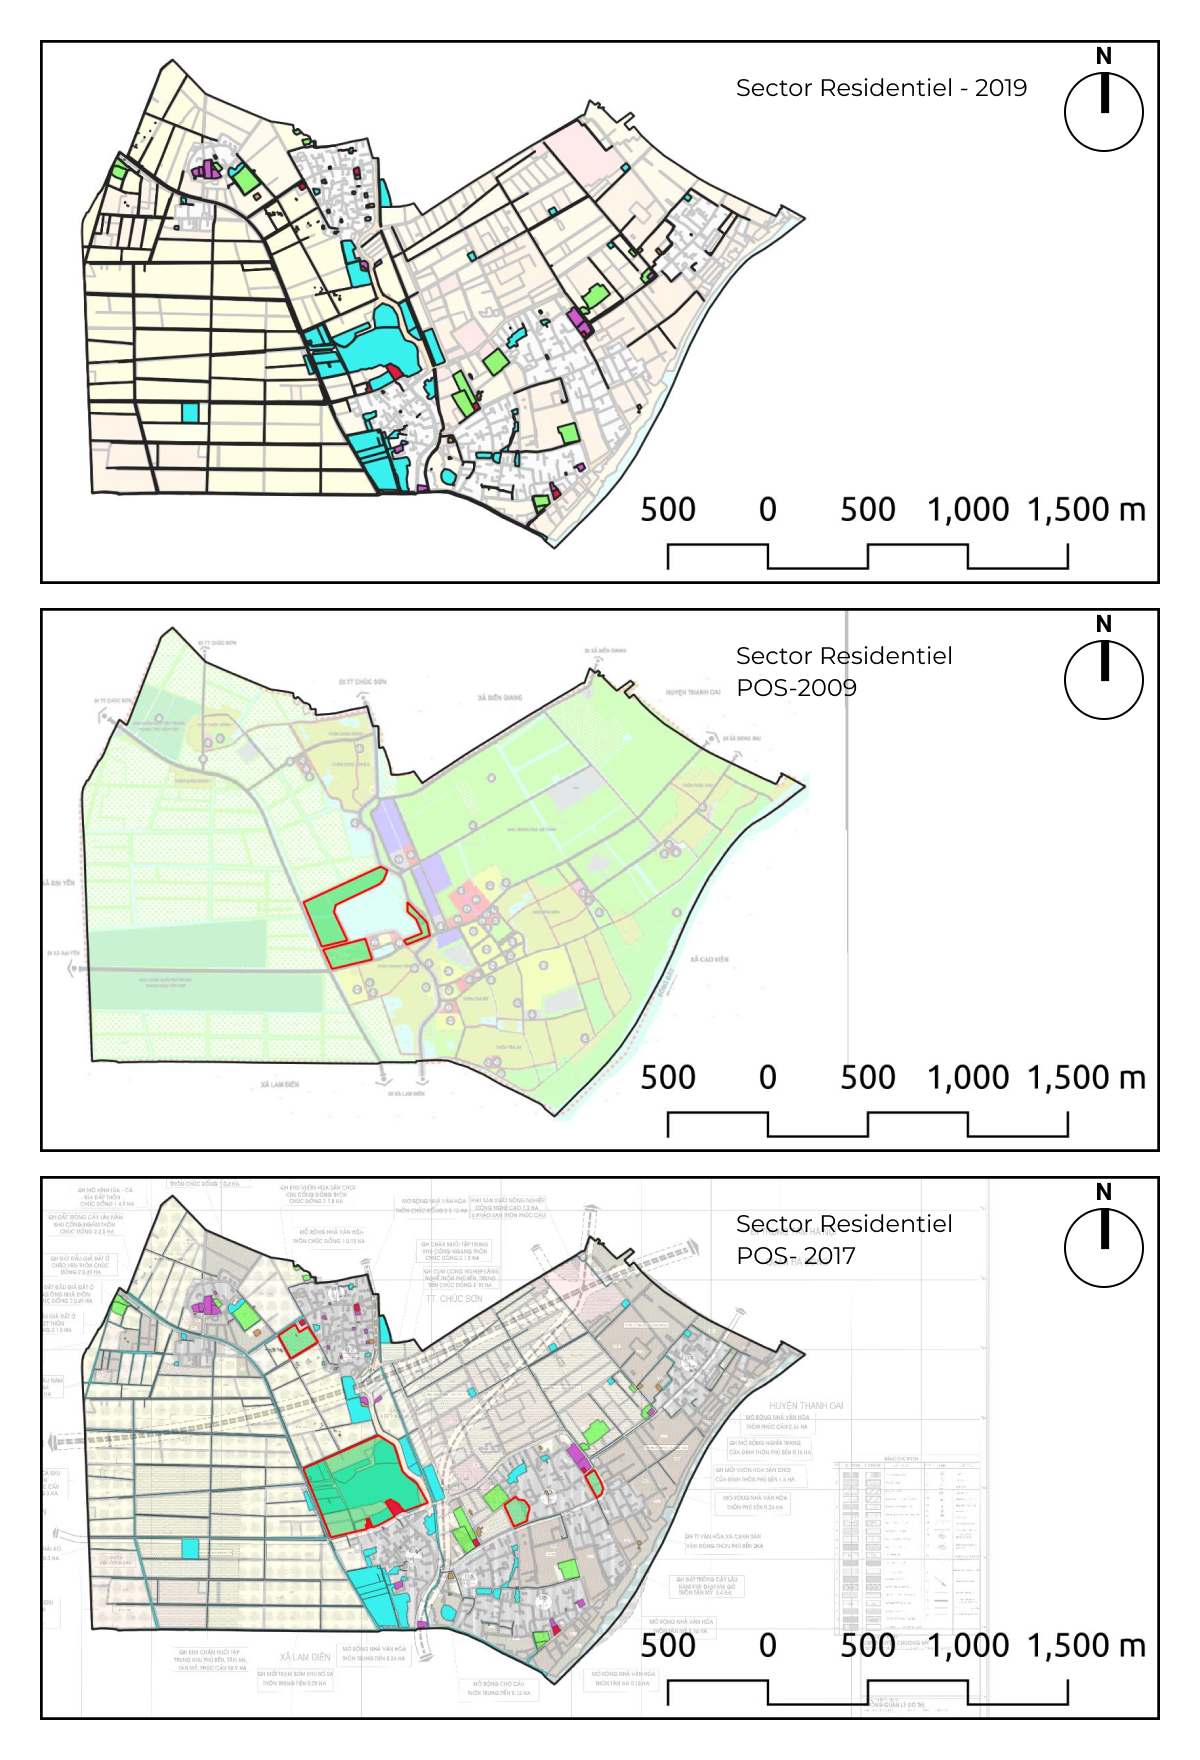
\includegraphics[width=15cm]{Graphic/TC6-QH-Xanh.jpg}
\caption{Khu o qua cac ban do}
\end{figure}
\clearpage

\subsection {Quy hoạch không gian sản xuất Nông nghiệp}
\section {Khảo sát xã hội học về biến đổi KGKTCQ dưới ảnh hưởng NTM tại khu vực nghiên cứu}
\end{document}